\documentclass{beamer}
\usepackage[utf8]{inputenc}
\usepackage[T1]{fontenc}
\usepackage{lmodern}
\usepackage[english]{babel}
\usepackage{lsfolien}
\usepackage{hyperref}
\usepackage{graphicx}

\myfootline{System Modelling and Semantic Web -- Summer Term 2022}{Cecilia Graiff}

\title{Hands on Systematic Innovation\\
	Problem Solving Tools - Knowledge
	\vskip1em}

\subtitle{Presentation in the Module 10-202-2312}

\author{Cecilia Graiff}

\date{June 28^{th}, 2022}


\begin{document}

	\begin{frame}[plain]
		\maketitle
	\end{frame}

	\section{Motivation}
	\begin{frame}{Introduction}
        \begin{itemize}
				\item In today's world, access to a huge amount of (not only) business and management data is easily granted to everyone
				\item Systematic innovation methods are built around a subject-action-object (=noun-verb-noun) template
				\item The access to knowledge databases is only the first step to a long series of actions
			\end{itemize}
		\end{frame}
		
	\begin{frame}{Levels of Abstraction}
	        \begin{figure}
				\centering
				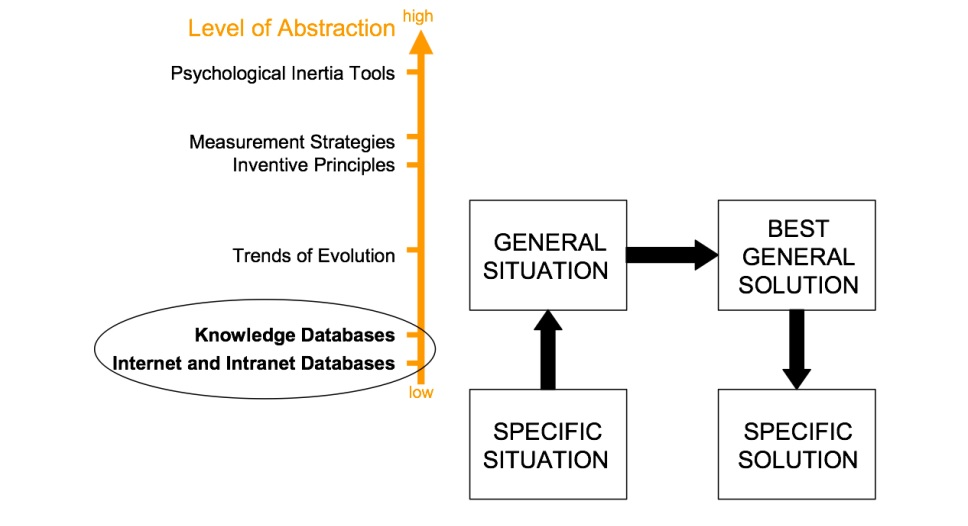
\includegraphics[scale=0.4]{figure_3.jpg}
				\caption{Levels of Abstraction in the Systematic Innovation Process (Hands on Systematic Innovation for Business and Management, Darrell Mann)}
			\end{figure}
	\end{frame}
		
	\begin{frame}{Handling Knowledge}
        \begin{itemize}
				\item Accessing Knowledge
				\item Using Knowledge Search Tools
				\item Beyond Knowledge: Context and Wisdom
				\item Knowledge Management
			\end{itemize}

	\end{frame}

	\section{Accessing Knowledge}   
	\begin{frame}{Accessing Knowledge}
        \begin{itemize}
				\item Knowledge sharing is better achieved when solutions are arranged in terms of functions
				\item From the business point of view: shift from selling washing powder to selling cleaned clothes
				\item From the technical side: What are the function words?
				\item Focus on the connection between things (=verbs), not on things \emph{per se} (=nouns)!
			\end{itemize}

	\end{frame}

	\begin{frame}{Function Words}
	\begin{itemize}
			\item Accomplishment Verbs
				\begin{itemize}
					\item achieve, become, elect, improve, ...
				\end{itemize}
			\item Creative Verbs
			    \begin{itemize}
					\item act, create, customize, draw, ...
				\end{itemize}
			\item Clerical or Detail Verbs
				\begin{itemize}
					\item approve, arrange, host, implement, ...
				\end{itemize}
			\item Communication Verbs
			    \begin{itemize}
					\item address, advertize, entertain, inform, ...
				\end{itemize}
			\item Financial Verbs
				\begin{itemize}
					\item administrate, compute, budget, calculate, ...
				\end{itemize}
	\end{itemize}
	\end{frame}
	
	\begin{frame}{Function Words}
	\begin{itemize}
		 \item Helping Verbs
			     \begin{itemize}
					\item aid, clarify, coach, fortify, ...
				 \end{itemize} 
		 \item Management Verbs
			     \begin{itemize}
					\item administer, chair, handle, hire, ...
				 \end{itemize} 
		 \item Research Verbs
			     \begin{itemize}
					\item apply, check, examine, explore, ...
				 \end{itemize} 
		 \item Technical Verbs
			     \begin{itemize}
					\item adjust, alter, assemble, fabricate, ...
				 \end{itemize} 
		\item Negative Verbs
			     \begin{itemize}
					\item corrupt, damage, destroy, hire, ...
				 \end{itemize} 
	    \end{itemize}
	\end{frame}
	
	\section{Research Tools}
	 \begin{frame}{Information versus Time}
	        \begin{figure}
				\centering
				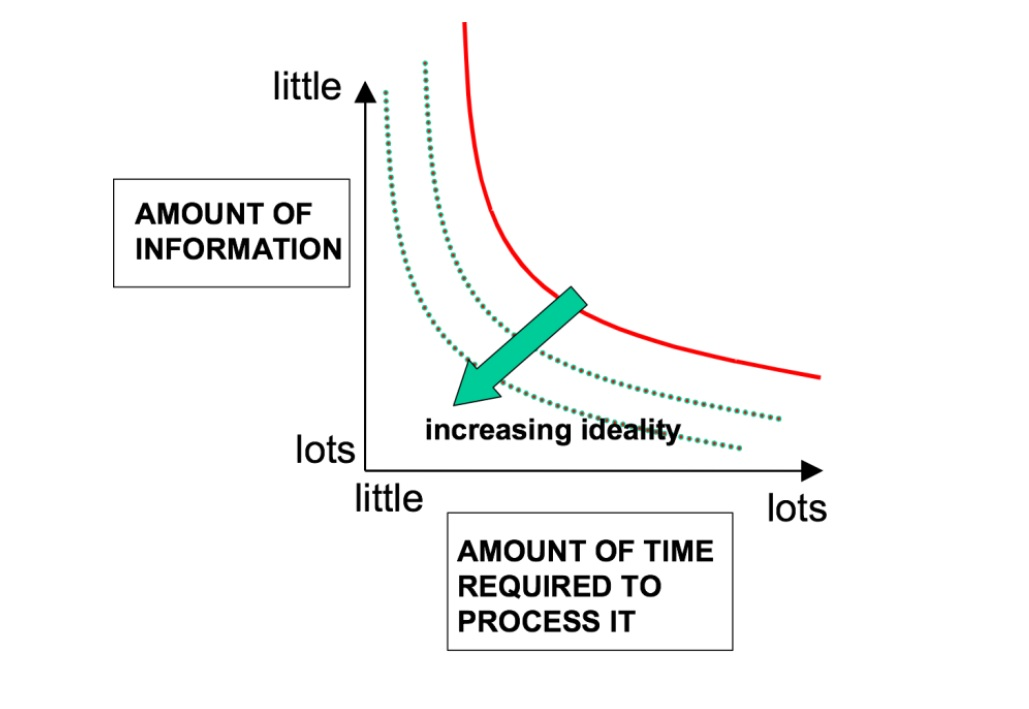
\includegraphics[scale=0.4]{graph_1.jpg}
				\caption{The Information versus Time Conflict (Hands on Systematic Innovation for Business and Management, Darrell Mann)}
			\end{figure}
	    \end{frame}

	\begin{frame}{Knowledge Search Tools}
		\begin{itemize}
			\item Search Engines
			\item Semantic Search Tools
			\item User-Defined Context Search Tools
			\item Intelligent Agent-Based Search Tools
		\end{itemize}
	\end{frame}

	\begin{frame}{Search Engines}
		\begin{itemize}
		    \item Example: Google
			\item What you need probably is in the top 10% or 20%
			\item The distance between words is an important parameter
		\end{itemize}
	\end{frame}



	\begin{frame}{Semantic Search Tools}
		\begin{itemize}
			\item Example: Goldfire/Knowledgist Product from Invention Machine
			\item Based on the subject-action-object template: given a sentence, these tools extract subject elements, action elements, and object elements.
		\end{itemize}
	\end{frame}
	
	\begin{frame}{User-Defined Context Search Tools}
	    \begin{itemize}
	        \item The first two tools do not consider the context of the search
	        \item Context Search Tools are built around context defined or user defined knowledge structures, like taxonomies or ontologies
	        \item Problem: classifications mostly are ambiguous
	        \item Latest generation tools try to overcome this problem by allowing concepts to migrate from one niche to another according to the user's wish of changing context
	    \end{itemize}
	\end{frame}

	\begin{frame}{Intelligent Agent-Based Search Tools}
		\begin{itemize}
		    \item Bottom-up rules
		    \item The tool learns about the context by watching what the user does
		    \item One (very simple) example could be Amazon
		\end{itemize}
	\end{frame}

    \section{Wisdom}
	\begin{frame}{Context and Wisdom}
	 \begin{figure}
				\centering
				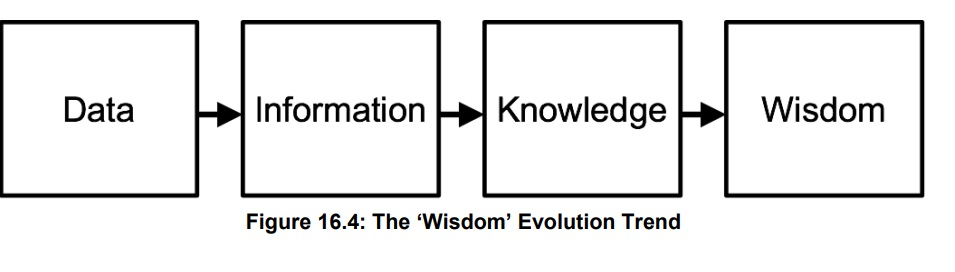
\includegraphics[scale=0.5]{figure_2.jpg}
				\caption{The 'Wisdom' Evolution Trend (Hands on Systematic Innovation for Business and Management, Darrell Mann)}
	    \end{figure}
	\end{frame}
	
		\begin{frame}{Context and Wisdom}
	 \begin{block}{What is Wisdom?}
	     "Wisdom may be thought of as the successful application of knowledge; the successful application of knowledge means setting that knowledge into the specific and unique context of the situation." (Darrell Mann)
	     
	 \end{block}
	\end{frame}
	
	\section{Knowledge Management}
	\begin{frame}{Knowledge Management}
		\begin{itemize}
		    \item The ideas and concepts mentioned in this presentation allow the creation of an universally applicable knowledge framework
		    \item "someone, somewhere has already solved this problem"
		\end{itemize}
	\end{frame}
	
		\begin{frame}{Knowledge Management for Business Models}
		\begin{itemize}
		    \item What are the characteristics of successful business models for the management and protection of knowledge?
		    \begin{enumerate}
		        \item Trust
		        \item Faith in the power of self-organization system
		        \item There should be no knowledge management departments
		        \item The ability to forget knowledge that is no longer relevant
		    \end{enumerate}
		    
		\end{itemize}
	\end{frame}
	
		\begin{frame}{Rules for the application of this method}
		\begin{itemize}
		    \item "Someone, somewhere already solved this problem" is not always applicable. Therefore, the method offers many research strategies to assist in the search of other solutions; Most importantly, they rely on functions.
		    \item Since technology is proceeding fast, many research tools are provided. Choosing the most useful one is a very important step in the process.
		    \item There are no short-cuts and there is no substitute context-driven application of knowledge!
		\end{itemize}
	\end{frame}
	
\end{document}
